\PassOptionsToPackage{unicode=true}{hyperref} % options for packages loaded elsewhere
\PassOptionsToPackage{hyphens}{url}
%
\documentclass[]{article}
\usepackage{lmodern}
\usepackage{amssymb,amsmath}
\usepackage{ifxetex,ifluatex}
\usepackage{fixltx2e} % provides \textsubscript
\ifnum 0\ifxetex 1\fi\ifluatex 1\fi=0 % if pdftex
  \usepackage[T1]{fontenc}
  \usepackage[utf8]{inputenc}
  \usepackage{textcomp} % provides euro and other symbols
\else % if luatex or xelatex
  \usepackage{unicode-math}
  \defaultfontfeatures{Ligatures=TeX,Scale=MatchLowercase}
\fi
% use upquote if available, for straight quotes in verbatim environments
\IfFileExists{upquote.sty}{\usepackage{upquote}}{}
% use microtype if available
\IfFileExists{microtype.sty}{%
\usepackage[]{microtype}
\UseMicrotypeSet[protrusion]{basicmath} % disable protrusion for tt fonts
}{}
\IfFileExists{parskip.sty}{%
\usepackage{parskip}
}{% else
\setlength{\parindent}{0pt}
\setlength{\parskip}{6pt plus 2pt minus 1pt}
}
\usepackage{hyperref}
\hypersetup{
            pdftitle={Análise de Regressão},
            pdfborder={0 0 0},
            breaklinks=true}
\urlstyle{same}  % don't use monospace font for urls
\usepackage[margin=1in]{geometry}
\usepackage{color}
\usepackage{fancyvrb}
\newcommand{\VerbBar}{|}
\newcommand{\VERB}{\Verb[commandchars=\\\{\}]}
\DefineVerbatimEnvironment{Highlighting}{Verbatim}{commandchars=\\\{\}}
% Add ',fontsize=\small' for more characters per line
\usepackage{framed}
\definecolor{shadecolor}{RGB}{248,248,248}
\newenvironment{Shaded}{\begin{snugshade}}{\end{snugshade}}
\newcommand{\AlertTok}[1]{\textcolor[rgb]{0.94,0.16,0.16}{#1}}
\newcommand{\AnnotationTok}[1]{\textcolor[rgb]{0.56,0.35,0.01}{\textbf{\textit{#1}}}}
\newcommand{\AttributeTok}[1]{\textcolor[rgb]{0.77,0.63,0.00}{#1}}
\newcommand{\BaseNTok}[1]{\textcolor[rgb]{0.00,0.00,0.81}{#1}}
\newcommand{\BuiltInTok}[1]{#1}
\newcommand{\CharTok}[1]{\textcolor[rgb]{0.31,0.60,0.02}{#1}}
\newcommand{\CommentTok}[1]{\textcolor[rgb]{0.56,0.35,0.01}{\textit{#1}}}
\newcommand{\CommentVarTok}[1]{\textcolor[rgb]{0.56,0.35,0.01}{\textbf{\textit{#1}}}}
\newcommand{\ConstantTok}[1]{\textcolor[rgb]{0.00,0.00,0.00}{#1}}
\newcommand{\ControlFlowTok}[1]{\textcolor[rgb]{0.13,0.29,0.53}{\textbf{#1}}}
\newcommand{\DataTypeTok}[1]{\textcolor[rgb]{0.13,0.29,0.53}{#1}}
\newcommand{\DecValTok}[1]{\textcolor[rgb]{0.00,0.00,0.81}{#1}}
\newcommand{\DocumentationTok}[1]{\textcolor[rgb]{0.56,0.35,0.01}{\textbf{\textit{#1}}}}
\newcommand{\ErrorTok}[1]{\textcolor[rgb]{0.64,0.00,0.00}{\textbf{#1}}}
\newcommand{\ExtensionTok}[1]{#1}
\newcommand{\FloatTok}[1]{\textcolor[rgb]{0.00,0.00,0.81}{#1}}
\newcommand{\FunctionTok}[1]{\textcolor[rgb]{0.00,0.00,0.00}{#1}}
\newcommand{\ImportTok}[1]{#1}
\newcommand{\InformationTok}[1]{\textcolor[rgb]{0.56,0.35,0.01}{\textbf{\textit{#1}}}}
\newcommand{\KeywordTok}[1]{\textcolor[rgb]{0.13,0.29,0.53}{\textbf{#1}}}
\newcommand{\NormalTok}[1]{#1}
\newcommand{\OperatorTok}[1]{\textcolor[rgb]{0.81,0.36,0.00}{\textbf{#1}}}
\newcommand{\OtherTok}[1]{\textcolor[rgb]{0.56,0.35,0.01}{#1}}
\newcommand{\PreprocessorTok}[1]{\textcolor[rgb]{0.56,0.35,0.01}{\textit{#1}}}
\newcommand{\RegionMarkerTok}[1]{#1}
\newcommand{\SpecialCharTok}[1]{\textcolor[rgb]{0.00,0.00,0.00}{#1}}
\newcommand{\SpecialStringTok}[1]{\textcolor[rgb]{0.31,0.60,0.02}{#1}}
\newcommand{\StringTok}[1]{\textcolor[rgb]{0.31,0.60,0.02}{#1}}
\newcommand{\VariableTok}[1]{\textcolor[rgb]{0.00,0.00,0.00}{#1}}
\newcommand{\VerbatimStringTok}[1]{\textcolor[rgb]{0.31,0.60,0.02}{#1}}
\newcommand{\WarningTok}[1]{\textcolor[rgb]{0.56,0.35,0.01}{\textbf{\textit{#1}}}}
\usepackage{graphicx,grffile}
\makeatletter
\def\maxwidth{\ifdim\Gin@nat@width>\linewidth\linewidth\else\Gin@nat@width\fi}
\def\maxheight{\ifdim\Gin@nat@height>\textheight\textheight\else\Gin@nat@height\fi}
\makeatother
% Scale images if necessary, so that they will not overflow the page
% margins by default, and it is still possible to overwrite the defaults
% using explicit options in \includegraphics[width, height, ...]{}
\setkeys{Gin}{width=\maxwidth,height=\maxheight,keepaspectratio}
\setlength{\emergencystretch}{3em}  % prevent overfull lines
\providecommand{\tightlist}{%
  \setlength{\itemsep}{0pt}\setlength{\parskip}{0pt}}
\setcounter{secnumdepth}{0}
% Redefines (sub)paragraphs to behave more like sections
\ifx\paragraph\undefined\else
\let\oldparagraph\paragraph
\renewcommand{\paragraph}[1]{\oldparagraph{#1}\mbox{}}
\fi
\ifx\subparagraph\undefined\else
\let\oldsubparagraph\subparagraph
\renewcommand{\subparagraph}[1]{\oldsubparagraph{#1}\mbox{}}
\fi

% set default figure placement to htbp
\makeatletter
\def\fps@figure{htbp}
\makeatother


\title{Análise de Regressão}
\author{}
\date{\vspace{-2.5em}}

\begin{document}
\maketitle

\newcommand{\bfbeta}{\hbox{$\boldsymbol \beta$}}
\newcommand{\bfY}{\textbf{Y}}

Modelos de Regressão são utilizados para descrever o relacionamento de
uma variável \(y\) com outra (ou outras) variável \(x\), por meio de uma
relação matemática da forma
\[y = f(x;\hbox{$\boldsymbol \beta$}) + \textrm{erro}.\] Quando a função
\(f\) é do tipo
\[f(x;\hbox{$\boldsymbol \beta$}) = \beta_0 + \beta_1 x,\]
\(\hbox{$\boldsymbol \beta$}=(\beta_0,\beta_1) \in \mathbb{R}^2\),
tem-se um modelo de regressão linear simples. A variável \(x\) é a
variável independente do modelo, enquanto \(y\) depende das variações de
\(x\), e é chamada de variável resposta. Assim, o modelo de regressão é
chamado de simples quando envolve uma relação causal entre duas
variáveis, \(x\) e \(y\). O modelo de regressão é múltiplo quando
envolve uma relação causal entre mais de duas variáveis. Ou seja, quando
a variação da resposta \(y\) pode ser explicada por mais de uma variável
independente, \(x_1,...,x_p\), que são também denominadas variáveis
explicativas ou covariáveis.

Modelos de regressão podem ser aplicados em vários tipos de probelas.

1 - Em problemas em que se deseja realizar previsões sobre o
comportamento futuro de algum fenômeno, extrapolando-se para o futuro as
relações de causa e efeito observados no passado.

2 - Quando é desejado observar efeitos causados por uma variável \(x\)
sobre outra variável (sobre a variável resposta) em decorrência de
alterações introduzidas em seus valores.

\textbf{Modelos de Regressão Linear Simples}

Considere a variável Diferencial de Pressão e a variável Temperatura
Interna dos dados do moinho de cimento. Vamos assumir que y represente a
variável Diferencial de Pressão (variável resposta) e x represente a
variável Temperatura Interna do moinho (variável independente). Vamos
considerar os valores das variáveis observados em um período de um dia
(28/01/2019), considerando intervalos entre as coletas de três horas
(3h). Essas dados são coletados a cada 30min, no entanto esses valores
podem conter uma dependência ao longo do tempo, que pode ser amenizada
considerando um intervalo maior entre as coletas.

\begin{Shaded}
\begin{Highlighting}[]
\NormalTok{lab=}\KeywordTok{which}\NormalTok{(x}\OperatorTok{==}\NormalTok{x)}
\KeywordTok{ggplot}\NormalTok{(df, }\KeywordTok{aes}\NormalTok{(}\DataTypeTok{x=}\NormalTok{ x, }\DataTypeTok{y=}\NormalTok{ y, }\DataTypeTok{colour=}\StringTok{"green"}\NormalTok{, }\DataTypeTok{label=}\NormalTok{lab))}\OperatorTok{+}
\StringTok{  }\KeywordTok{geom_point}\NormalTok{() }\OperatorTok{+}\KeywordTok{geom_text}\NormalTok{(}\KeywordTok{aes}\NormalTok{(}\DataTypeTok{label=}\NormalTok{lab),}\DataTypeTok{hjust=}\DecValTok{0}\NormalTok{, }\DataTypeTok{vjust=}\DecValTok{0}\NormalTok{)}
\end{Highlighting}
\end{Shaded}

\includegraphics{RegLinear_files/figure-latex/unnamed-chunk-7-1.pdf}

\begin{Shaded}
\begin{Highlighting}[]
\KeywordTok{plot}\NormalTok{(x,y, }\DataTypeTok{xlab=}\StringTok{"MILL IN TEMP (C) PV"}\NormalTok{, }\DataTypeTok{ylab=}\StringTok{"CEMENT MILL DP (mbar) PV"}\NormalTok{)}
\end{Highlighting}
\end{Shaded}

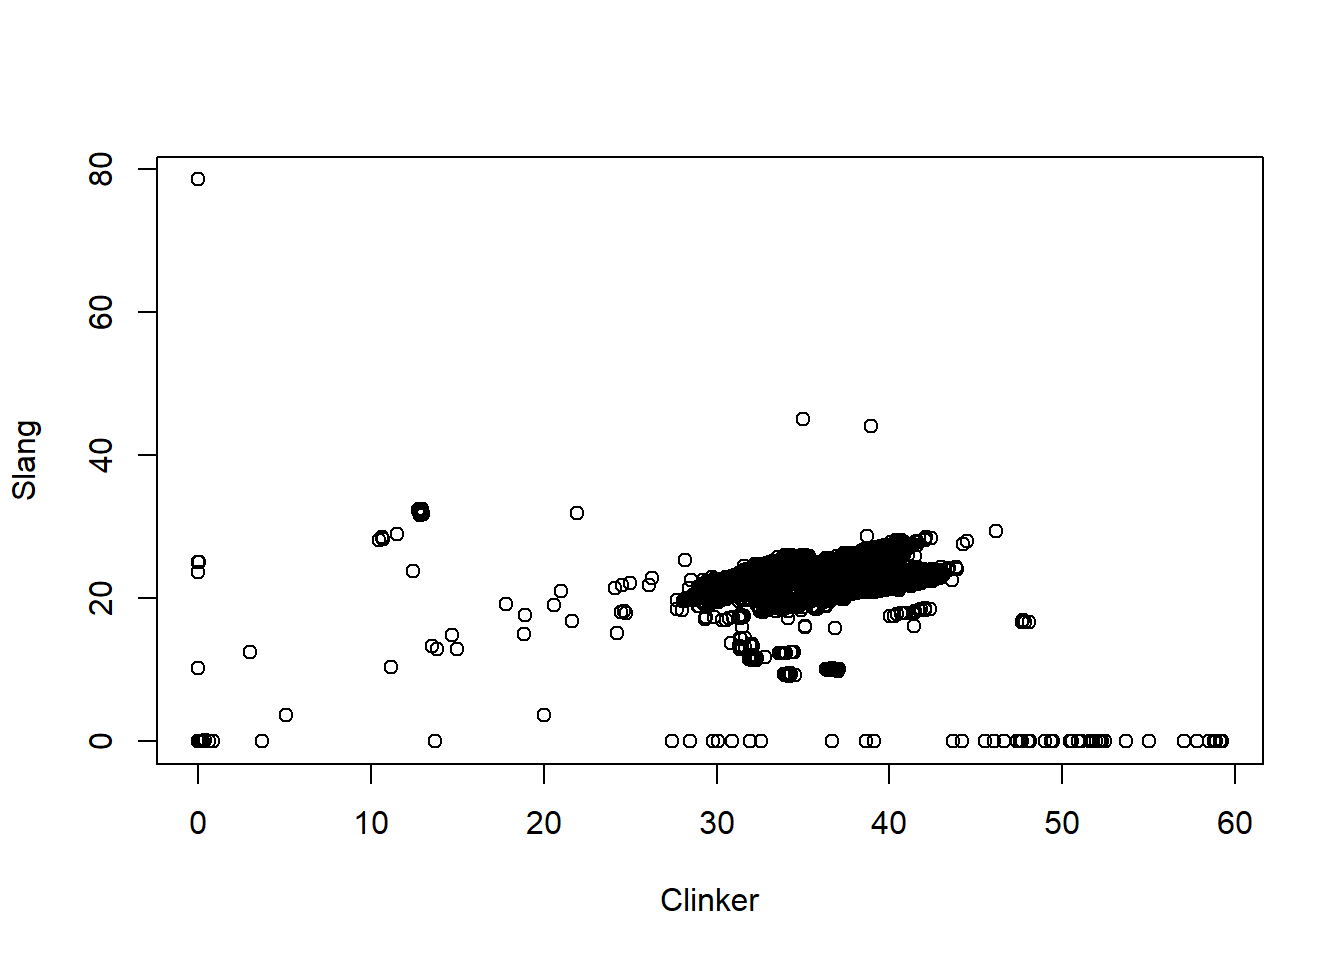
\includegraphics{RegLinear_files/figure-latex/unnamed-chunk-8-1.pdf}

Note que parece existir uma associação entre as a variáveis, pois a
medida que x aumenta, a variável y parece tender a também aumentar. Se a
relação existe, em geral, é desejado saber qual é a função que pode
descrever o relacionamento. Neste caso, pode-se fazer a suposição
inicial de que esta função seja uma reta, ou seja, pode-se supor que um
modelo de regressão linear seja apropriado. Assim, o interesse é
aproximar os dados a melhor reta possível, para tentar prever o
comportamento da variável \(x\) em função de \(y\).

\textbf{Modelos de Regressão Linear Múltiplo}

O modelo de regressão linear múltiplo é expresso pela função linear:
\[y = \beta_0 + \beta_1 x_1 + ... + \beta_p x_p + \varepsilon\] em que:

\(y\) é a variável resposta (variável dependente no modelo)

\(x_1,...,x_p\) são as covariáveis (variáveis independentes ou
explicativas), supostamente independentes entre si;

\(\beta_0,...,\beta_p\) são os coeficientes da regressão;

\(\varepsilon\) é o erro aleatório.

Agora, considere uma amostra \(y_1,...,y_n\) de \(y\) em que cada
\(y_i\) está associado às \(p\) variáveis explicativas,
\(x_i,x_{i1},...,x_{ip}\), \(i=1,..,n\), assim pelo modelo
\[y_i = \beta_0 + \beta_1x_{i1} + ... + \beta_px_{ip} + \varepsilon_i\,,\]
\(i=1,..,n\) e \(n>p\), que pode ser visto como um modelo de regressão
linear amostral.

No modelo de regressão usual, os \(\varepsilon_i\)'s são variáveis
aleatórias sujeitas as seguintes condições:

\begin{itemize}
\tightlist
\item
  \(E[\varepsilon_i] = 0\);

  \begin{itemize}
  \tightlist
  \item
    \(Var(\varepsilon_i) = \sigma^2\);
  \item
    \(Cov(\varepsilon_i,\varepsilon_j) = 0 \,, \forall i \neq j\,, j=1,...,n\).
  \end{itemize}
\end{itemize}

Note que, \(x_{i1},...,x_{ip}\) são variáveis numéricas, não são
variáveis aleatórias. No entanto, cada \(y_i\) depende da quantidade
aleatória \(\varepsilon_i\) e portanto é uma variável aleatória. Assim,
a média de \(y_i\) é dada por:
\[ E[y_i] = E[\beta_0 + \beta_1x_{i1} + ... + \beta_px_{ip} + \varepsilon_i] = \beta_0 + \beta_1x_{i1} + ... + \beta_px_{ip}\]
e a variância é dada por:
\[ Var(y_i) = Var(\beta_0 + \beta_1x_{i1} + ... + \beta_px_{ip} + \varepsilon_i) = \sigma^2, \ \ \  \forall i .\]

Usando a notação matricial, o modelo é dado por:

\[
\begin{pmatrix}
y_1 \\ y_2 \\ \vdots \\ y_n
\end{pmatrix}
=
\begin{pmatrix}
1 & x_{11} & x_{12} & \cdots & x_{1p} \\
1 & x_{11} & x_{12} & \cdots & x_{1p} \\
\vdots & \vdots & \vdots & \ddots & \vdots \\
1 & x_{n1} & x_{n2} & \cdots & x_{np} \\
\end{pmatrix}
\begin{pmatrix}
\beta_0 \\ \beta_1 \\ \vdots \\ \beta_p
\end{pmatrix}
+
\begin{pmatrix}
\varepsilon_1 \\ \varepsilon_2 \\ \vdots \\ \varepsilon_n
\end{pmatrix}
\Rightarrow
\textbf{Y}= X  \beta+   \varepsilon
\]

A matriz \(X\) de dimensão \(n \times (p+1)\) e chamada de matriz de
regressão quando \(rank[X] = p+1\), e é chamada de matriz de
delineamento quando \(rank[X] = r < p+1\). A coluna de \(1\)'s na matriz
refere-se ao intercepto, \(\beta_0\). O vetor \(Y\) de dimensão
\(n \times 1\) contém as variáveis \(y_1,..,y_n\), \(\beta\) é o vetor
de dimensão \((p+1) \times 1\) dos coeficientes de regressão e
\(\varepsilon\) é o vetor de erros aleatórios de dimensão
\(n \times 1\).

Conseqüentemente, \[E[{ \bf Y}] = E[X{ \bf \beta}+{ \bf \varepsilon}]\]
e
\[Var({ \bf Y}) = Var(X{ \bf \beta}+{ \bf \varepsilon}) = \sigma^2 I_n\,,\]
em que \(I_n\) é a matriz identidade de dimensão \(n \times n\).

\textbf{Estimação por mínimos quadrados}

O método de mínimos quadrados (\(MMQ\)) aplica-se somente aos parâmetros
\({ \bf \beta} = (\beta_0,\beta_1,...,\beta_p)\), e é frequentemente
aplicado em situações em que não se dispõe de mais especificações, além
das que já foram feitas, sobre os erros. Este método consiste em estimar
\(\widehat{{ \bf \beta}} = (\widehat{\beta_0},\widehat{\beta_1},...,\widehat{\beta_p})\)
por \({ \bf \beta} = (\beta_0,\beta_1,...,\beta_p)\) de modo que o vetor
de valor esperado \(E[{ \bf Y}] = X{ \bf \beta}\) esteja tão perto
quanto possível do vetor de observações \({ \bf y}\) de \({ \bf Y}\). Ou
seja, os estimadores de mínimos quadrados de
\(\beta_0,\beta_1,...,\beta_p\) devem minimizar a soma dos quadrados dos
erros, dada por:

\[U({ \bf \beta}) = \displaystyle\sum_{i=1}^n\varepsilon_i^2 = \displaystyle\sum_{i=1}^n(y - \beta_0 - \beta_1x_{i1} - ... - \beta_px_{ip})^2 = 
{ \bf \varepsilon}^T{ \bf \varepsilon}\]

Nota que \(U({ \bf \beta})\) pode ser expresso por:
\[U({ \bf \beta}) = { \bf Y}^T{ \bf Y} - { \bf \beta}^TX^T{ \bf Y} - { \bf Y}^TX{ \bf \beta} + { \bf \beta}^TX^TX{ \bf \beta} = { \bf Y}^T{ \bf Y} - 2{ \bf \beta}^TX^T{ \bf Y} + { \bf \beta}^TX^TX{ \bf \beta}\]

Derivando \(U({ \bf \beta})\) com respeito a \({ \bf \beta}\) e
igualando a zero, temos:
\[\dfrac{\partial U({ \bf \beta})}{\partial { \bf \beta}} = - 2X^T{ \bf Y} + 2X^TX\widehat{{ \bf \beta}} = 0 \,,\]
que resulta em: \[X^TX{ \bf \beta} = X^T{ \bf Y} \,,\] denominadas
equações normais.

Se \(rank[X] = p+1\), \(X^TX\) é positiva definida e, portanto,
inversível (não-singular). Assim, as equações normais possuem uma
solução única dada por:
\[\widehat{{ \bf \beta}} = (X^TX)^{-1}X^T{ \bf Y} \,,\] em que
\(\widehat{{ \bf \beta}}\) é o estimador de mínimos quadrados (\(EMQ\))
de \(\beta\).

O modelo de regressão ajustado, correspondente ao vetor, \({ \bf Y}\), é
dado por:
\[\widehat{{ \bf Y}} = X\widehat{{ \bf \beta}} = X(X^TX)^{-1}X^T{ \bf Y} = H{ \bf Y}\,.\]

A matriz \(H = X(X^TX)^{-1}X^T\) de dimensão \(n \times n\) é geralmente
chamada de matriz chapéu. Essa matriz possui algumas propriedades
importantes que são enunciadas no teorema a seguir.

Teorema \(3.1\): Suponha que X é uma matriz \(n \times (p+1)\) de
\(rank\) completo \(p+1\). Então,

\begin{itemize}
\item
  \(H\) e (\(I_n - H\)) são simétricas e idempotente;
\item
  \(rank[I_n - H] = Tr[I_n - H] = n-(p+1) = n-p-1\);
\item
  \(HX = X\).
\end{itemize}

\end{document}
